\chapter{\ifenglish Background Knowledge and Theory\else ทฤษฎีที่เกี่ยวข้อง\fi}

\hspace{1.27cm}การทำโครงงาน เริ่มต้นด้วยการศึกษาค้นคว้า ทฤษฎีที่เกี่ยวข้อง หรือ งานวิจัย/โครงงาน ที่เคยมีผู้นำเสนอไว้แล้ว ซึ่งเนื้อหาในบทนี้ก็จะเกี่ยวกับการอธิบายถึงสิ่งที่เกี่ยวข้องกับโครงงาน เพื่อให้ผู้อ่านเข้าใจเนื้อหาในบทถัดๆ ไปได้ง่ายขึ้น

\section{ระบบฐานข้อมูล (Database System)}
\hspace{1.27cm}ระบบฐานข้อมูล (Database System) หมายถึงโครงสร้างสารสนเทศที่ประกอบด้วย รายละเอียดของข้อมูลที่เกี่ยวข้องกันที่จะนำมาใช้ในระบบต่าง ๆ ร่วมกัน  ซึ่่งผู้ใช้สามารถจัดการกับ
ข้อมูลได้ในลักษณะต่าง ๆ ทั้งเพิ่ม ลบ หรือแก้ไขตลอดจนการเรียกดูข้อมูล ส่วนใหญ่จะเป็นการประยุกต์นำเอาระบบคอมพิวเตอร์เข้ามาช่วยในการจัดการฐานข้อมูล

ระบบฐานข้อมูล มีคำศัพท์ต่างๆที่เกี่ยวข้องดังนี้

\begin{enumerate}
  \hangindent=2em \hangafter=1
  \item เอนทิตี้ (Entity) หมายถึงสิ่งที่เราสนใจจะเก็บข้อมูล เช่น นักศึกษา อาจารย์ วิชาการ หรือห้องเรียน
  \item แอตทริบิวต์ (Attribute) หมายถึงคุณสมบัติของเอนทิตี้ เช่น ชื่อ นามสกุล หรือรหัสนักศึกษา
  \item ความสัมพันธ์ (Relationship) หมายถึงความสัมพันธ์ระหว่างเอนทิตี้ โดยที่เอนทิตี้หนึ่งสามารถมีความสัมพันธ์กับเอนทิตี้อีกเอนทิตี้หนึ่งได้ เช่น นักศึกษาสามารถลงทะเบียนเรียนในหลายวิชา และวิชาใด ๆ ก็สามารถมีนักศึกษาหลายคนลงทะเบียนเรียนได้
  \item คีย์หลัก (Primary Key) หมายถึงคีย์ที่ใช้เพื่อระบุเอนทิตี้นั้น ๆ อย่างชัดเจน และไม่สามารถซ้ำกันได้  
  \item คีย์นอก (Foreign Key) หมายถึงคีย์ที่เป็นคีย์หลักของเอนทิตี้หนึ่ง และเป็นคีย์ที่อยู่ในเอนทิตี้อีกเอนทิตี้หนึ่ง  
\end{enumerate}



\section{ไมโครเซอร์วิส (Microservices)}
\hspace{1.27cm}Microservice\cite{microservice} หรือ Microservice Architecture คือสถาปัตยกรรมการออกแบบ Service หรือก็คือออกแบบซอฟต์แวร์ โดยการที่ในชื่อมีคำว่า Micro นำหน้าอยู่ก็เพราะว่าเป็นการออกแบบที่ทำให้ Service มีขนาดเล็กเพื่อแก้ไขจุดด้อยของสถาปัตยกรรมการออกแบบอื่นๆ 

\subsection{Monolithic VS Microservice}
\hspace{1.27cm}หาก Microservice เป็นการออกแบบ Service ให้มีขนาดเล็ก การจะเทียบให้เห็นภาพชัดเจนที่สุดก็ต้องเทียบกับ Monolithic ที่เป็นระบบที่มีขนาดใหญ่ โดย Monolithic จะเป็นระบบที่มีการทำงานทั้งหมดอยู่ใน Service เดียว
% Subsection 1 text
% \clearpage
\begin{figure}[H] % 'H' forces placement exactly here
% \begin{figure}[ht] % 'ht' means place it approximately here
  \centering
  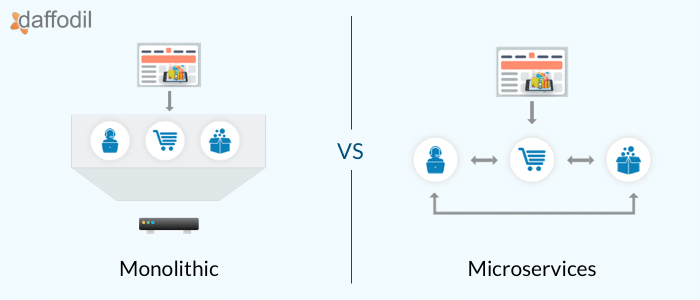
\includegraphics[width=\linewidth, keepaspectratio]{pictures/monolithic-vs-microservices.png}
  \caption[Poem]{รูปจาก nsights.daffodilsw.com}
  % \label{fig:monolithic-vs-microservices}
\end{figure}


\subsubsection{ความแตกต่างระหว่าง Monolithic และ Microservice}
\begin{itemize}
  \item \textbf{Monolithic} เป็นชื่อของสถาปัตยกรรมการออกแบบซอฟต์แวร์หรือ Service ที่มีคนใช้งานเป็นจำนวนมากและมีมาอย่างยาวนาน โดยเป็นลักษณะของระบบที่การทำงานทุกอย่างจะรวมอยู่ในกลุ่มก้อนเดียวกัน และใช้งาน Database เดียวกัน (อย่างในภาพจะเห็นว่าเป็นเว็บไซต์ขายสินค้าที่มีฟังก์ชันจัดการผู้ใช้, ตะกร้าสินค้า และการส่งสินค้า รวมอยู่ด้วยกัน และใช้ฐานข้อมูลเดียวกัน)
  \item \textbf{Microservice}  จะออกแบบโดยแยกการทำงานที่รวมกันเป็นก้อนใหญ่ๆของแบบ Monolithic ออกมาให้เล็กลงโดยอาจจะแยกตามบริการหรือตามฟังก์ชันการทำงานเลยก็ได้ (จากในภาพฟังก์ชันทั้งสามอย่างจะแยกออกจากกัน และไม่ได้ใช้ฐานข้อมูลเดียวกันในการเก็บข้อมูลอีกต่อไป เพราะแต่ละฟังก์ชันหรือบริการที่แยกออกมามีฐานข้อมูลเป็นของตัวเอง และสามารถติดต่อกันได้ผ่าน API )
\end{itemize}




\subsubsection{ข้อดีและข้อเสียของ Microservice}
\begin{itemize}
  \item ข้อดี
  \begin{enumerate}
    \item การทำงานหลักแต่ละส่วนของระบบ ถ้าเป็นไปได้ควรแยกออกเป็น service แต่ละอัน เช่นจัดการสินค้า กับจัดการการซื้อสินค้าก็แยกกันไปเลย
    \item มีที่เก็บข้อมูลของตัวเอง
  \end{enumerate}
  \item ข้อเสีย
  \begin{enumerate}
    \item การจัดการระบบที่มีหลาย service อาจจะทำให้การจัดการระบบทำได้ยากขึ้น
    \item การทำงานของระบบที่แยกออกมาอาจจะทำให้การทำงานของระบบช้าลง
  \end{enumerate}
\end{itemize}
\clearpage
\section{RabbitMQ}
\hspace{1.27cm}RabbitMQ \cite{rabbitmq}ซอฟต์แวร์ที่เป็นตัวกลางรับส่งข้อความระหว่างแอปพลิเคชันต่างๆ ผู้ไปรับรับข้อความจากผู้ส่ง (แอปพลิเคชันหนึ่ง) เก็บไว้รอการคัดแยก และส่งต่อให้ผู้รับ (แอปพลิเคชันอีกแอปพลิเคชันหนึ่ง) เหมาะสำหรับการทำแอปพลิเคชันที่ต้องมีการจัดคิวในการส่งข้อความ ระบบที่เป็นไมโครเซอร์วิสเอาไว้สื่อสารกันได้อย่างมีประสิทธิภาพ ทำให้สามารถแบ่งงานขนาดใหญ่เป็นงานย่อยๆ และส่งไปยังระบบอื่นๆ เพื่อประมวลผลได้นั่นเอง
\begin{figure}[H] % 'H' forces placement exactly here
  % \begin{figure}[ht] % 'ht' means place it approximately here
    \centering
    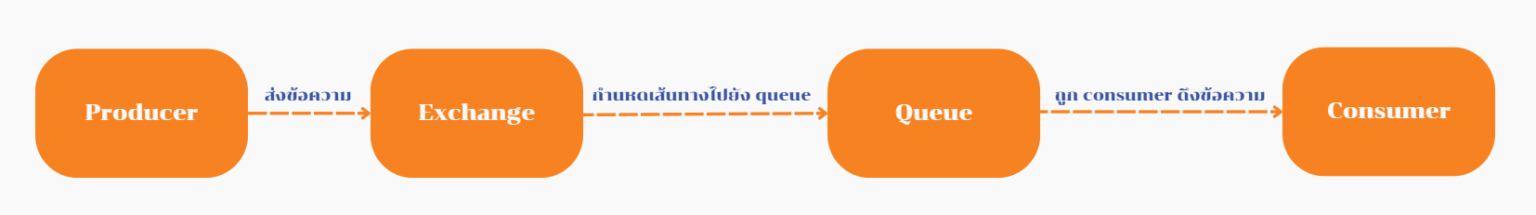
\includegraphics[width=\linewidth, keepaspectratio]{pictures/rabbitmq.png}
    \caption[Poem]{รูปจาก https://www.borntodev.com/2024/06/09/rabbitmq-nodejs/}
    \label{fig:rabbitmq}
\end{figure}
  \subsection{คำศัพท์ต่างๆที่เกี่ยวข้อง}
  \begin{itemize}
    \item \textbf{Producer} คือ ผู้ส่งข้อความ
    \item \textbf{Consumer} คือ ผู้รับข้อความ
    \item \textbf{Queue} คือ คิวข้อความ
    \item \textbf{Exchange} คือ ตัวกลางในการส่งข้อความ
    \item \textbf{Binding} คือ การเชื่อมต่อระหว่าง Exchange กับ Queue
    \item \textbf{Channel} คือ ช่องสื่อสารระหว่าง Producer และ Consumer
    \item \textbf{Connection} คือ การเชื่อมต่อระหว่าง RabbitMQ กับ Producer และ Consumer
  \end{itemize}
% Section 3 text. The dielectric constant\index{dielectric constant}
% at the air-metal interface determines
% the resonance shift\index{resonance shift} as absorption or capture occurs
% is shown in Equation~\eqref{eq:dielectric}:

% \begin{equation}\label{eq:dielectric}
% k_1=\frac{\omega}{c({1/\varepsilon_m + 1/\varepsilon_i})^{1/2}}=k_2=\frac{\omega
% \sin(\theta)\varepsilon_\mathit{air}^{1/2}}{c}
% \end{equation}

% \noindent
% where $\omega$ is the frequency of the plasmon, $c$ is the speed of
% light, $\varepsilon_m$ is the dielectric constant of the metal,
% $\varepsilon_i$ is the dielectric constant of neighboring insulator,
% and $\varepsilon_\mathit{air}$ is the dielectric constant of air.

\section{Framework ที่ใช้ในการพัฒนา}
\hspace{1.27cm}Framework อาจหมายถึง ชุดคำสั่ง เครื่องมือ หรือโครงสร้างอย่างใดอย่างหนึ่ง
ที่สร้างขึ้นมาเพื่ออำนวยความสะดวกแก่ผู้ใช้งาน ซึ่ง Framework มีหลายประเภท หลายแบบ และจะมีวิธีการใช้ที่คล้ายๆกัน
\subsection{Next.js}
\begin{figure}[H] % 'H' forces placement exactly here
  % \begin{figure}[ht] % 'ht' means place it approximately here
    \centering
    
\includegraphics[width=60mm, keepaspectratio ]{pictures/nextjs.png}
    \caption[Poem]{รูปจาก https://medium.com/geekculture/why-should-you-learn-next-js-in-2021-what-are-the-benefits-8292d79bc50c}
    \label{fig:nextjs}
\end{figure}
\hspace{1.27cm}Next.js\cite{Nextjs} คือ JavaScript webapps framework ถูกสร้างขึ้น on top จาก library อย่าง React, Webpack, และ Babel ขึ้นมาอีกที มีจุดเด่นคือ เป็น SSR (server-side rendering) ตั้งแต่ต้น
\subsubsection{ข้อดีของ Next.js}
\begin{itemize}
  \item สามารถทำ SSR ได้ง่าย
  \item มีการจัดการ SEO ที่ดี
  \item Hot reload เวลาเราแก้ไขไฟล์ หน้าเว็บของเราจะถูก refresh โดยอัตโนมัติ 
  \item Project Structure ที่ชัดเจนที่ถูกออกแบบมาให้เรียบร้อยแล้ว
  \item Routing ด้วยความที่มี project structure การทำ routingจึงสามารถ auto routing ได้
\end{itemize}


\subsection{ElysiaJs}
\begin{figure}[H] % 'H' forces placement exactly here
  % \begin{figure}[ht] % 'ht' means place it approximately here
    \centering
    
\includegraphics[width=80mm, keepaspectratio ]{pictures/elysia.jpg}
    \caption[Poem]{รูปจาก https://sadewawicak25.medium.com/file-upload-and-security-validation-on-elysia-js-2-d6c57b023441}
    \label{fig:elysia}
\end{figure}
\hspace{1.27cm}ElysiaJS\cite{ElysiaJs} คือ Framework ในการพัฒนา API ด้วยภาษา Typescript โดยมีจุดเด่นคือ ความเร็วที่เร็วกว่า Express ถึง 21 เท่า (เนื่องจาก ElysiaJS มีการใช้ Bun เป็น Runtime) และอีกจุดเด่นคือ End-to-end Type Safety หรือชนิดของข้อมูลที่ชัดเจน ทำให้เวลาเราทำงานร่วมกับผู้อื่นสามารถทำได้สะดวกมากยิ่งขึ้น เพราะไม่ต้องมาทะเลาะกันเรื่องชนิดของข้อมูลที่ส่งให้กัน อีกทั้งยังมี Community ที่เติบโตเร็ว


\subsection{Gin}
\begin{figure}[H]
  \centering
  
\includegraphics[width=40mm, keepaspectratio ]{pictures/gin.png}
  \caption[Poem]{รูปจาก https://www.askme.co.th/article/what-is-docker/}
  \label{fig:gin}
\end{figure}
\hspace{1.27cm}Gin\cite{Gin101} เป็น web framework ที่เขียนด้วยภาษา golang ที่ถูกพัฒนาต่อมาจาก Martini API ที่หยุดพัฒนาไปแล้ว โดย Gin จะใช้ customized httprouter ทำให้มีประสิทธิภาพด้านความเร็วที่สูงมากกว่า Martini ถึง 40 \cite{GinFeature}เท่า ทำให้มีperformance กับ productivity ที่ดี 

\subsubsection{Feature สำคัญของ Gin มีดังนี้ }
\begin{itemize}
  \item \textbf{JSON validation} สามารถแปลงและตรวจสอบ JSON ของ HTTP request
  \item \textbf{Routes grouping} จัดกลุ่ม routes ของ request ว่า request ไหนต้องมีการ authorization หรือไม่จำเป็นต้องมี การแยก request ด้วย version ของ API โดยสามารถจัดกลุ่มได้อย่างไม่จำกัด และไม่กระทบกับประสิทธิภาพ
  \item \textbf{Middleware support} incoming HTTP request จะถูกจัดการด้วย chain ของ middleware และ action สุดท้าย
  \item \textbf{Rendering build-in} ง่ายสำหรับสร้าง API ที่ render เป็น JSON, XML และ HTML
  \item \textbf{Error management} สามารถจัดการ error ที่เกิดขึ้นในระดับ application และ HTTP ได้
\end{itemize}

\subsection{Docker}
\begin{figure}[H]
  \centering
  
\includegraphics[width=100mm, keepaspectratio ]{pictures/docker.png}
  \caption[Poem]{รูปจาก https://www.docker.com/}
  \label{fig:docker}
\end{figure}

\hspace{1.27cm}Docker เป็นแพลตฟอร์มโอเพนซอร์สที่ช่วยในการสร้าง ทดสอบ และปรับใช้แอปพลิเคชันในรูปแบบของคอนเทนเนอร์ คอนเทนเนอร์เป็นสภาพแวดล้อมที่แยกจากกันที่สามารถรันแอปพลิเคชันได้ โดยที่ไม่ต้องกังวลเกี่ยวกับการกำหนดค่าหรือการติดตั้งซอฟต์แวร์เพิ่มเติมในระบบปฏิบัติการหลักของเซิร์ฟเวอร์ที่ใช้

\hspace{0.8cm}สิ่งที่ทำให้ Docker แตกต่างจากเทคโนโลยีอื่นๆ เช่น Virtual Machines (VMs) คือ Docker ใช้ Kernel ของระบบปฏิบัติการเดียวกันในการรันคอนเทนเนอร์แต่ละตัว ทำให้มีประสิทธิภาพในการใช้งานทรัพยากรสูงขึ้น และทำให้คอนเทนเนอร์ใช้เวลาในการเริ่มต้นที่รวดเร็ว

\subsubsection{องค์ประกอบหลักของ Docker}
\begin{itemize}
  \item \textbf{Docker Engine} เป็นซอฟต์แวร์ที่รันอยู่เบื้องหลังซึ่งทำหน้าที่สร้างและจัดการคอนเทนเนอร์ในระบบ มันมีองค์ประกอบย่อย 2 ส่วนที่สำคัญ ได้แก่
  \begin{enumerate}
    \item Docker Daemon (dockerd): เป็นโปรแกรมหลักที่รันอยู่เบื้องหลังและรับคำสั่งจาก Docker Client ผ่าน API โดย Daemon จะจัดการทุกอย่างที่เกี่ยวข้องกับคอนเทนเนอร์ เช่น การสร้าง, การเริ่มต้น, การหยุด, และการลบคอนเทนเนอร์
    \item Docker CLI (docker): คือส่วนที่ผู้ใช้ใช้ในการสั่งการ Docker ผ่านคำสั่งต่างๆ ผ่าน Command Line Interface เช่น การสร้างคอนเทนเนอร์ (docker run), การสร้างอิมเมจ (docker build), และการจัดการเครือข่าย (docker network)
  \end{enumerate}
  \item \textbf{Docker Image} คือไฟล์แบบคงที่ที่บรรจุโค้ดแอปพลิเคชันและทุกสิ่งที่แอปพลิเคชันนั้นต้องการในการรัน เช่น ไลบรารี, การตั้งค่า, และไฟล์ระบบ Image ถูกสร้างจากไฟล์ที่เรียกว่า Dockerfile ซึ่งเป็นไฟล์ที่กำหนดขั้นตอนในการติดตั้งและตั้งค่าแอปพลิเคชัน
  
  \hspace{1cm}\textbf{Dockerfile Syntax} ที่ใช้ในการสร้าง Image มีคำสั่งที่เป็นลำดับขั้นตอน ยกตัวอย่างเช่น
  \hspace{1cm}\begin{enumerate}
    \item FROM: ระบุ Image เบื้องต้น เช่น Ubuntu, Alpine หรือ Node.js
    \item RUN: รันคำสั่งใน Image เช่น การติดตั้งแพ็คเกจ
    \item COPY/ADD: คัดลอกไฟล์จากโฮสต์เข้าสู่ Image
    \item CMD/ENTRYPOINT: กำหนดคำสั่งที่รันเมื่อคอนเทนเนอร์เริ่มทำงาน
  \end{enumerate}
  \item \textbf{Docker Container} คือ สิ่งที่ถูกสร้างจาก Docker Image และเป็นสภาพแวดล้อมที่แยกจากกันที่สามารถรันแอปพลิเคชันได้โดยมีคุณสมบัติดังนี้
  \item \begin{enumerate}
    \item แยกการทำงานจากระบบปฏิบัติการโฮสต์ แต่ยังใช้เคอร์เนลร่วมกัน
    \item สามารถสร้าง, ลบ, หยุด, และรีสตาร์ทได้อย่างง่ายดาย
    \item สามารถแชร์ทรัพยากรเครือข่ายและไฟล์ระหว่างคอนเทนเนอร์ต่างๆ ได้
  \end{enumerate}
\end{itemize}

\subsubsection{ความแตกต่างระหว่าง Docker กับ Virtual Machines}
\tolerance= 9999
\begin{table}[H]
  \centering
  \caption{เปรียบเทียบคุณสมบัติของ Docker และ Virtual Machine (VM)}
  \label{tab:docker-vm}

  \renewcommand{\arraystretch}{1.3} % Adjust row spacing
  \setlength{\extrarowheight}{3pt}  % Extra row height for better spacing
  \setlength{\tabcolsep}{8pt}       % Adjust column padding

  
  \begin{tabular}{|>{\raggedright\arraybackslash}p{3cm}|>{\raggedright\arraybackslash}p{5cm}|>{\raggedright\arraybackslash}p{5cm}|}
    % Balanced column widths
      \hline
      \rowcolor{gray!20} 
      \textbf{คุณสมบัติ} & \textbf{Docker} & \textbf{Virtual Machine (VM)} \\
      \hline
      การใช้เคอร์เนล & ใช้เคอร์เนลของระบบปฏิบัติการโฮสต์ & จำลองระบบปฏิบัติการเต็มรูปแบบ \\
      \hline
      ขนาดไฟล์ & ขนาดเล็ก & ขนาดใหญ่ \\
      \hline
      เวลาเริ่มต้น & เริ่มต้นได้อย่างรวดเร็ว & ใช้เวลามากขึ้น \\
      \hline
      การใช้ทรัพยากร & ใช้ทรัพยากรน้อย & ใช้ทรัพยากรมาก \\
      \hline
      ความยืดหยุ่น & เหมาะสำหรับแอปพลิเคชันแบบไมโครเซอร์วิส & เหมาะสำหรับการจำลองระบบขนาดใหญ่ \\
      \hline
      การแยกทรัพยากร & แยกการทำงานในระดับแอปพลิเคชัน & แยกระบบปฏิบัติการทั้งหมด \\
      \hline
  \end{tabular}
\end{table}

\hspace{1.27cm}โดยรวมแล้ว Docker เหมาะสำหรับการรันแอปพลิเคชันที่ต้องการความยืดหยุ่นในการปรับใช้และทรัพยากรที่มีข้อจำกัด ในขณะที่ VM เหมาะกับการรันระบบที่ต้องการการแยกสภาพแวดล้อมอย่างสมบูรณ์ เช่น การรันหลายระบบปฏิบัติการในเครื่องเดียวกัน



% define a command that produces some filler text, the lorem ipsum.
% \newcommand{\loremipsum}{
%   \textit{Lorem ipsum dolor sit amet, consectetur adipisicing elit, sed do
%   eiusmod tempor incididunt ut labore et dolore magna aliqua. Ut enim ad
%   minim veniam, quis nostrud exercitation ullamco laboris nisi ut
%   aliquip ex ea commodo consequat. Duis aute irure dolor in
%   reprehenderit in voluptate velit esse cillum dolore eu fugiat nulla
%   pariatur. Excepteur sint occaecat cupidatat non proident, sunt in
%   culpa qui officia deserunt mollit anim id est laborum.}\par}

% \begin{figure}
%   \centering

%   \fbox{
%      \parbox{.6\textwidth}{\loremipsum}
%   }

%   % To include an image in the figure, say myimage.pdf, you could use
%   % the following code. Look up the documentation for the package
%   % graphicx for more information.
%   % \includegraphics[width=\textwidth]{myimage}

%   \caption[Sample figure]{This figure is a sample containing \gls{lorem ipsum},
%   showing you how you can include figures and glossary in your report.
%   You can specify a shorter caption that will appear in the List of Figures.}
%   \label{fig:sample-figure}
% \end{figure}

% Using \verb.\label. and \verb.\ref. commands allows us to refer to
% figures easily. If we can refer to Figures
% \ref{fig:walrus} and \ref{fig:sample-figure} by name in the {\LaTeX}
% source code, then we will not need to update the code that refers to it
% even if the placement or ordering of the figures changes.

% \loremipsum\loremipsum

% This code demonstrates how to get a landscape table or figure. It
% uses the package lscape to turn everything but the page number into
% landscape orientation. Everything should be included within an
% \afterpage{ .... } to avoid causing a page break too early.
% \afterpage{
%   \begin{landscape}
%   \begin{table}
%     \caption{Sample landscape table}
%     \label{tab:sample-table}

%     \centering

%     \begin{tabular}{c||c|c}
%         Year & A & B \\
%         \hline\hline
%         1989 & 12 & 23 \\
%         1990 & 4 & 9 \\
%         1991 & 3 & 6 \\
%     \end{tabular}
%   \end{table}
%   \end{landscape}
% }

% \loremipsum\loremipsum\loremipsum

\section{Overfull hbox}

When the \verb.semifinal. option is passed to the \verb.cpecmu. document class,
any line that is longer than the line width, i.e., an overfull hbox, will be
highlighted with a black solid rule:
\begin{center}
\begin{minipage}{10em}
juxtaposition
\end{minipage}
\end{center}

\section{\ifenglish%
\ifcpe CPE \else ISNE \fi knowledge used, applied, or integrated in this project
\else%
ความรู้ตามหลักสูตรซึ่งถูกนำมาใช้หรือบูรณาการในโครงงาน
\fi
}

อธิบายถึงความรู้ และแนวทางการนำความรู้ต่างๆ ที่ได้เรียนตามหลักสูตร ซึ่งถูกนำมาใช้ในโครงงาน

\section{\ifenglish%
Extracurricular knowledge used, applied, or integrated in this project
\else%
ความรู้นอกหลักสูตรซึ่งถูกนำมาใช้หรือบูรณาการในโครงงาน
\fi
}

อธิบายถึงความรู้ต่างๆ ที่เรียนรู้ด้วยตนเอง และแนวทางการนำความรู้เหล่านั้นมาใช้ในโครงงาน
